% The master copy of this demo dissertation is held on my filespace
% on the cl file serve (/homes/mr/teaching/demodissert/)

% Last updated by MR on 2 August 2001

\documentclass[12pt,twoside,notitlepage]{report}

\usepackage{a4}
\usepackage{verbatim}
\usepackage{units}
\usepackage{hyperref}
\usepackage{array}
\usepackage{listings}
\usepackage{parskip}
\usepackage{color}
\usepackage[usenames,dvipsnames]{xcolor}
\usepackage[noline,plain]{algorithm2e}
\usepackage{minibox}
\usepackage{amsfonts}
\usepackage{graphicx}
\usepackage{float}
\usepackage{soul}
\usepackage{hyperref}
\usepackage{paralist}

% \usepackage{dejavu}
% \usepackage{courier}
\usepackage[T1]{fontenc}

\input{epsf}                            % to allow postscript inclusions
% On thor and CUS read top of file:
%     /opt/TeX/lib/texmf/tex/dvips/epsf.sty
% On CL machines read:
%     /usr/lib/tex/macros/dvips/epsf.tex


\raggedbottom                           % try to avoid widows and orphans
\sloppy
\clubpenalty1000%
\widowpenalty1000%

\addtolength{\oddsidemargin}{6mm}       % adjust margins
\addtolength{\evensidemargin}{-8mm}

\renewcommand{\baselinestretch}{1.1}    % adjust line spacing to make
                                        % more readable
                                        
\newcommand{\strAuthor}{David Brazdil}
\newcommand{\strCollege}{Trinity Hall}
\newcommand{\strTitle}{Taint-based Data Flow Analysis on Android}
\newcommand{\strExamination}{Computer Science Tripos, Part II}
\newcommand{\strYear}{June 2013}
\newcommand{\strSupervisor}{Dr A. Beresford}

\newcommand{\centerbox}[1] {
	\begin{center}
	\begin{footnotesize}
	\begin{tabular}{l}
		#1
	\end{tabular}
	\end{footnotesize}
	\end{center}
}
\newcommand{\asm}[1] {\texttt{#1}}
\newcommand{\asmExtra}[1] {\texttt{\hl{#1}}}

\newcommand{\tick}{$\checkmark$}
\newcommand{\cross}{$\times$}

\setlength{\intextsep}{10pt}

\definecolor{lightGreen}{HTML}{E3FFD5}
\sethlcolor{lightGreen}

\title{\strTitle}
\author{\strAuthor}

\begin{document}

\bibliographystyle{plain}

\lstset{
	language=Java,
	tabsize=2,
	basicstyle=\ttfamily\scriptsize,
	escapeinside=\`\`, %{\%*}{*)},
	captionpos=b,
	keywordstyle=\color[rgb]{0,0,1},
    commentstyle=\color[rgb]{0.133,0.545,0.133},
    stringstyle=\color[rgb]{0.627,0.126,0.941},	
}

%%%%%%%%%%%%%%%%%%%%%%%%%%%%%%%%%%%%%%%%%%%%%%%%%%%%%%%%%%%%%%%%%%%%%%%%
% Title


\pagestyle{empty}

\hfill{\LARGE \bf \strAuthor}

\vspace*{60mm}
\begin{center}
\Huge
{\bf \strTitle} \\
\vspace*{5mm}
\strExamination \\
\vspace*{5mm}
\strCollege \\
\vspace*{5mm}
\today  % today's date
\end{center}

\cleardoublepage

%%%%%%%%%%%%%%%%%%%%%%%%%%%%%%%%%%%%%%%%%%%%%%%%%%%%%%%%%%%%%%%%%%%%%%%%%%%%%%
% Proforma, table of contents and list of figures

\setcounter{page}{1}
\pagenumbering{roman}
\pagestyle{plain}

\chapter*{Proforma}

{\large
\begin{tabular}{ll}
Name:               & \bf \strAuthor                       \\
College:            & \bf \strCollege                     \\
Project Title:      & \bf \strTitle \\
Examination:        & \bf \strExamination, \strYear        \\
Word Count:         & \bf 1587\footnotemark[1] \\
Project Originator: & \strSupervisor                    \\
Supervisor:         & \strSupervisor                    \\ 
\end{tabular}
}
\footnotetext[1]{This word count was computed
by {\tt detex -n diss.tex | tr -cd '0-9A-Za-z $\tt\backslash$n' | wc -w}
}
\stepcounter{footnote}


\section*{Original Aims of the Project}

To write a demonstration dissertation\footnote{A normal footnote without the
complication of being in a table.} using \LaTeX\ to save
student's time when writing their own dissertations. The dissertation
should illustrate how to use the more common \LaTeX\ constructs. It
should include pictures and diagrams to show how these can be
incorporated into the dissertation.  It should contain the entire
\LaTeX\ source of the dissertation and the Makefile.  It should
explain how to construct an MSDOS disk of the dissertation in
Postscript format that can be used by the book shop for printing, and,
finally, it should have the prescribed layout and format of a diploma
dissertation.


\section*{Work Completed}

All that has been completed appears in this dissertation.

\section*{Special Difficulties}

Learning how to incorporate encapsulated postscript into a \LaTeX\
document on both CUS and Thor.
 
\newpage
\section*{Declaration}

I, [Name] of [College], being a candidate for Part II of the Computer
Science Tripos [or the Diploma in Computer Science], hereby declare
that this dissertation and the work described in it are my own work,
unaided except as may be specified below, and that the dissertation
does not contain material that has already been used to any substantial
extent for a comparable purpose.

\bigskip
\leftline{Signed [signature]}

\medskip
\leftline{Date [date]}

\cleardoublepage

\tableofcontents

\listoffigures

\newpage
\section*{Acknowledgments}

This document owes much to an earlier version written by Simon Moore
\cite{moore95}.  His help, encouragement and advice was greatly 
appreciated.

%%%%%%%%%%%%%%%%%%%%%%%%%%%%%%%%%%%%%%%%%%%%%%%%%%%%%%%%%%%%%%%%%%%%%%%
% now for the chapters

\cleardoublepage        % just to make sure before the page numbering
                        % is changed

\setcounter{page}{1}
\pagenumbering{arabic}
\pagestyle{headings}

\chapter{Introduction}

One out of three free apps spies on users: \url{http://www.huffingtonpost.com/alexandru-catalin-cosoi/one-out-of-three-free-and_b_3006729.html}

\cleardoublepage
\chapter{Preparation}

\section{Dalvik Virtual Machine}

Dalvik is an open-source virtual machine and an essential component of the Android operating system. It was developed specifically for use on mobile devices such as smartphones and tablets, and its design was optimized for running on battery-powered systems with low-performance processor and limited memory. 

Built around the Apache Harmony project, Dalvik runs programs that are compatible with a subset of the Java runtime framework. Applications for Dalvik are therefore typically written in Java, compiled to a set of JVM bytecode \emph{.class} files, and then converted to a single Dalvik-compatible \emph{.dex} file using tools in the Android SDK. With release 2.2, Dalvik introduced Just-In-Time compilation which significantly increased its performance and efficiency\footnote{\url{http://android-developers.blogspot.com/2010/05/dalvik-jit.html}}.

\subsection{Application Package Files}

Applications for Android are distributed in Application Package files (APK). These are ZIP files signed by the publisher, which contain:
\begin{inparaenum}[(i)]
\item the executable \emph{classes.dex} file,
\item application resources (images, UI layouts, ...),
\item native code binaries,
\item manifest.
\end{inparaenum}

The compulsory manifest file contains essential information about the application to the operating system. Among other things, this includes its unique package name, list of permissions requested by the application, and a list of all its entry points.

These files are stored on the device when applications are downloaded from the market or installed manually. System applications can be found in the \verb$/system/app$ folder, most applications installed by the user in \verb$/data/app$. Applications can also be moved to an SD card, in which case they are encrypted and accessed through virtual file-system. Either way, they can be retrieved from the device only with root access. The instrumented APK can be installed on any device, regardless of it being rooted or not. 

\subsection{Bytecode}

Dalvik bytecode is very similar to that of the Java Virtual Machine in the sense that it has a large set of rather high-level instructions, making the assembly nearly identical to the original source code unless obfuscation tools like ProGuard\footnote{\url{https://developer.android.com/tools/help/proguard.html}} are used. This makes analysis and reverse-engineering of applications a significantly easier task, and is also the reason why we will use both assembly and Java code examples freely.

\subsubsection{Registers}

Unlike the stack-based JVM, Dalvik uses a register-based programming model with 32-bit register width and variable-length instructions. 64-bit values are stored in two adjacent registers.

Each method can use up to 65,536 virtual registers. Actual mapping to hardware registers depends on the machine architecture. On a typical Android device, the first 16 virtual registers would map to the 16 registers available in the ARM instruction set, and rest would be stored in memory. Depending on their length, instructions can address either the first 16, first 256, or all 65k virtual registers. If an instruction needs to address a register out of the available range, the register contents are expected to get moved to a lower register first.

Dalvik also has a very powerful preload class verifier. It infers types of values stored in registers at every single point of computation, and uses this information to identify illegal access to resources, pointer arithmetic and other illegal operations. A class containing such instructions is rejected and the application terminated.

\subsubsection{Syntax of Assembly}
Assembly syntax used in this dissertation is mostly based on the official Dalvik assembly. It follows the \emph{dest-then-source} ordering of arguments, and instructions can contain immediate values, e.g. the instruction
		\centerbox{
			\asm{add-int/lit16 v2, v8, \#1234}
		}
adds 1234 to the value of register 8, and stores the result into register 2. 

Written rules of taint propagation will treat registers like variables. For example the following piece of code retrieves an element of an array pointed to by \verb$vArray$, and multiplies it by three.
	\begin{figure}[H]
		\centerbox{
			\asm{aget-int vElement, vArray, vIndex} \\
			\asm{mul-int/lit16 vResult, vElement, \#3}
		}
	\end{figure}

For better clarity, the first letters of register names will represent their origin. Names of registers used in the original code will start with \verb$r$, registers added for tainting with \verb$t$, and other with \verb$p$.

Register pairs forming a wide argument will be separated by a bar.
	\begin{figure}[H]
		\centerbox{
			\asm{move-wide rTo1 | rTo2, rFrom1 | rFrom2}
		}
	\end{figure}

\subsubsection{Instruction Variants}

To achieve higher code density, some Dalvik instructions come in several variants. They are semantically equivalent but they differ in size. A good example of this is the \verb$const$ instruction. Its variant \verb$const/16$ stores a 16-bit constant into a register addressed by an 8-bit number, fitting into 4 bytes. On the other hand, \verb$const/4$ fits into 2 bytes, but can only address registers in the 4-bit range and carry a 4-bit constant.

All variants of semantically equivalent instructions are parsed as the same instruction type in Dexter, and thus will be referred to  by the same name. During the reassembly phase, Dexter automatically outputs the most optimized variant of the instruction possible.

\section{Data Flow Analysis}
\label{section:DataFlowAnalysis}

\subsection{Taint Tags}

Different taint tracking systems choose different ways of representing taint tags. This fundamental choice has large effect on the overall design of the system, its capabilities and limits, as well as performance and memory overhead. The authors of TaintDroid decided to store taint tags as 32-bit integers where each bit represents one source of sensitive data. This is a very efficient and compact format, sufficient for the purposes of TaintDroid, but quickly reaches its limits as the functionality is extended. One of the challenges faced by the CleanOS project, which builds on TaintDroid, was the necessity to potentially track millions of taint sources. Their solution alters TaintDroid to store taint as a 32-bit pointer into an SQL database, which increases the number of trackable sources, but significantly impedes performance at the same time. 

For the sake of simplicity, Dexter adopts the same tag representation as TaintDroid, with one slight modification. As will be demonstrated later, identification of some sinks relies on distinguishing how certain objects were created. Hence upper bits of the tags are reserved to represent the potential of an object to create a particular type of sink if passed as an argument to some API calls. The meaning of each bit being set is summarized in table~\ref{table:TaintTagStorage_BitMeaning}.

\begin{table}
	\begin{center}
	\begin{tabular}{|c|l|l|}
		\firsthline
		\textbf{Bit} & \textbf{Constant name}        & \textbf{Description} \\
		\hline
		0            & \verb$TAINT_SOURCE_CONTACTS$  & contact information \\
		1            & \verb$TAINT_SOURCE_SMS$       & text message data \\
		2            & \verb$TAINT_SOURCE_CALL_LOG$  & call history information \\
		3            & \verb$TAINT_SOURCE_LOCATION$  & location information \\
		4            & \verb$TAINT_SOURCE_BROWSER$   & browser data, e.g. bookmarks \\
		5            & \verb$TAINT_SOURCE_DEVICE_ID$ & device ID, e.g. IMEI/phone number \\
		\hline
		29           & \verb$TAINT_SINK_FILE$        & file-system sink \\
		30           & \verb$TAINT_SINK_SOCKET$      & network sink \\
		31           & \verb$TAINT_SINK_OUT$         & standard console output sink \\
		\lasthline
	\end{tabular}
	\end{center}
	\caption{Meanings of bit flags of taint tags}
	\label{table:TaintTagStorage_BitMeaning}
\end{table}

\subsection{Tag Storage}

To store and propagate taint tags, Dexter must build an attribute system inside the modified application, so that every piece of data accessible by the executable code can carry a tag if necessary. The way these are stored differs for objects and for primitives. The crucial difference between these is that when a primitive is copied, operations on one of the copies do not effect the other ones, which means that there needs to be a tag storage for every copy. On the other hand, when a reference to an object is copied, operations on one of the copies are visible by dereferencing any of them, and so there should be only one taint tag per object, not per every copy of its reference. 

\subsubsection{Objects}
\label{section:TaintTagStorage_Objects}

Dexter allows to store one taint tag per object by adding a globally accessible hash map from object references to integers. The only two supported operation are:
\begin{description} 
\item \verb$int get(Object obj)$ \\
Returns the taint tag of given object. Returns zero when \verb$obj == null$.
\item \verb$void set(int taint, Object obj)$ \\
Adds taint to \verb$obj$ by OR-ing its existing entry with the first parameter. Does nothing when \verb$obj == null$.
\end{description}

In the following sections, the \verb$taint-get$ and \verb$taint-set$ pseudo-instructions (explained in section~\ref{section:Code_Pseudoinstructions}) will be used as a shorthand for calling the \verb$get$ and \verb$set$ methods of the hash map. Their syntax follows the signatures above:

	\begin{figure}[H]
		\centerbox{
			\asm{taint-get vResult, vObject} \\
			\asm{taint-set vAddedTaint, vObject}
		}
	\end{figure}

\subsubsection{Primitives}

\label{section:TaintStorage_Primitives}

In the case of primitives, Dexter needs to create taint storage space everywhere where a primitive might be stored, i.e. method code registers, and class fields and arrays of primitive types. Taint will also be temporarily stored for method arguments during a method call, but this will be discussed in section~\ref{section:TaintPropagation_MethodCalls_Internal}.

\begin{itemize}

\item \textbf{method code registers} \\
For every register that appears in the original method code, Dexter creates a new one that can be used for storing taint. This effectively doubles the number of used registers, which is why Dexter needs to perform constraint-solving register colouring during the assembly phase. Otherwise some instructions might not be able to address these new registers.

\item \textbf{internal class fields} \\
Classes defined inside the application's DEX file can be fully modified by Dexter. Hence, for every field of primitive type, a new field of type \verb$int$ is created, with a name that will not clash with any of the existing fields.

\item \textbf{external class fields} \\
Extra fields cannot be inserted into class defined outside the scope of the instrumented application, and therefore a different approach must be adopted. 
\begin{itemize}
\item static fields \\
A special class is created inside the application which contains one field of type \verb$int$ per every external static field that is accessed by the application. Taint tags are stored in these associated fields.

\item instance fields \\
It would be possible to create taint storage for every field inside every instance of an external class, for example by creating one global map from object references to integers per every accessed external instance field. However, it will be shown that it is actually necessary to assign the taint to the object itself, and thus storage space for these fields is not needed.

\item \textbf{arrays} \\
In Dexter's taint propagation logic, primitive arrays are equivalent to external instance fields, and therefore only one taint tag per array is stored.

\end{itemize}

\end{itemize}


\subsection{Principles of Taint Propagation}

Once taint storage is created, Dexter can insert extra instructions that will propagate taint as data are used. Dalvik supports 217 different opcodes, but these can be divided into groups that share the same propagation logic. General rule of thumb is that for every instruction, taint of all arguments should be acquired from their respective storage spaces, combined and stored to the taint storage of the result. Therefore, only a handful of examples will be presented here to illustrate the principle and to explain some of the subtleties.

The following sections will contain examples of instrumentation, first in Dalvik assembly and later in Java for better readability. Instrumentation will always be highlighted in green. 

\subsubsection{Constants}

Constants are created without any taint flags set. Zero should therefore be stored in the appropriate taint register.

	\begin{figure}[H]
		\centerbox{
			\asm{const rTo, \#num} \\
			\asmExtra{const tTo, \#0~~}
		}
	\end{figure}

\subsubsection{Instructions Combining Taint}

Arithmetic instructions are the simplest example of taint tag combination. Tags of the operands are OR-ed and this combined tag is assigned to the result of the original instruction.

	\begin{figure}[H]
		\centerbox{
			\asm{add-int rResult, rOpA, rOpB} \\
			\asmExtra{or-int tResult, tOpA, tOpB}
		}
	\end{figure}

\subsubsection{Instructions Operating on Wide Registers}

Taint for 64-bit primitives stored in wide register pairs is only stored in the taint register associated with the higher of the two original registers. This is safe because accessing only one of the registers as a single-width register is an illegal operation. Class containing such instruction will be rejected by Dalvik's preload class verifier.

	\begin{figure}[H]
		\centerbox{
			\asm{add-long rResult1 | rResult2, rOpA1 | rOpA2, rOpB1 | rOpB2} \\
			\asmExtra{or-int tResult1, tOpA1, tOpB1}
		}
	\end{figure}

\subsubsection{Instructions Throwing Exceptions}

Some of Dalvik instructions can throw exceptions, depending on the values of arguments. This is a form of implicit data flow which could potentially leak data. For example, integer division will throw \verb$ArithmeticException$ iff the divisor is zero, making this information deducible from the fact that the exception was thrown. Dexter deals with this by wrapping every such instruction in a try block, catching the exception, passing the correct taint to it and then throwing it again.

	\begin{figure}[H]
		\centerbox{
			\asmExtra{TRY (ArithmeticException $\Rightarrow$ CATCH\_ABC) \{} \\
			\asm{~~div-int rResult, rOpA, rOpB} \\
			\asmExtra{~~or-int tResult, tOpA, tOpB~~~~~~~~~~~~} \\
			\asmExtra{~~goto LABEL\_XYZ~~~~~~~~~~~~~~~~~~~~~~~~} \\
			\asmExtra{\}~~~~~~~~~~~~~~~~~~~~~~~~~~~~~~~~~~~~~~~} \\
			\asmExtra{CATCH\_ABC:~~~~~~~~~~~~~~~~~~~~~~~~~~~~~~} \\
			\asmExtra{move-exception pException~~~~~~~~~~~~~~~} \\
			\asmExtra{taint-set tOpB, pException~~~~~~~~~~~~~~} \\
			\asmExtra{throw pException~~~~~~~~~~~~~~~~~~~~~~~~} \\	
			\asmExtra{LABEL\_XYZ:~~~~~~~~~~~~~~~~~~~~~~~~~~~~~~}
		}
		\caption{Example instrumentation of the division instruction}
		\label{figure:TaintPropagation_ThrowingInstructions}
	\end{figure}

\subsection{Method Call Destination Decidability}
\label{section:TaintPropagation_DestDecision}

While the previous examples of propagation rules only dealt with tainting within the scope of one instrumented method, now we will focus on taint propagation when method calls are involved. 

The five types of method invocation supported by Dalvik are listed in table~\ref{table:TaintPropagation_MethodCallTypes}. Instrumentation of each will vary in slight details, but for tainting it will be more important to know whether a method call's target lies inside the DEX file, in which case taint should be propagated into the invoked method, or whether it jumps into untrackable and uninstrumentable code, and the invocation instrumentation should therefore assign taint conservatively, assuming the worst, i.e. that the method will spread taint everywhere it can.

\begin{table}[h]
	\begin{center}
	\begin{tabular}{|l|c|l|}
		\firsthline
		\textbf{Opcode}         & \footnotesize{\textbf{vtable}} & \textbf{Usage} \\
		\hline
		\verb$invoke-direct$    & \cross          & method a constructor or declared \verb$private$ \\
		\verb$invoke-static$    & \cross          & method declared \verb$static$ \\
		\hline
		\verb$invoke-virtual$   & \tick           & standard virtual method call \\
		\verb$invoke-interface$ & \tick           & method declared in an interface \\
		\verb$invoke-super$     & \tick           & call to closest parent implementing the method \\
		\lasthline
	\end{tabular}
	\end{center}
	\caption{Method call types supported by Dalvik}
	\label{table:TaintPropagation_MethodCallTypes}
\end{table}

Deciding the destination of a method call is trivial for \verb$invoke-direct$ instructions. The method signature, instruction's argument, always contains the name of the class implementing the method. Thus, it will perform an internal jump iff the referenced class is internal.

Only slightly more complicated is the case of a \verb$invoke-static$ call. The reason being that the method might not be implemented directly in the referenced class, but inherited from a parent, rendering the referenced class internality check insufficient. Dexter must check that the class indeed implements the method and recursively explore the parent if not.

\begin{figure}
	\centerline{	
		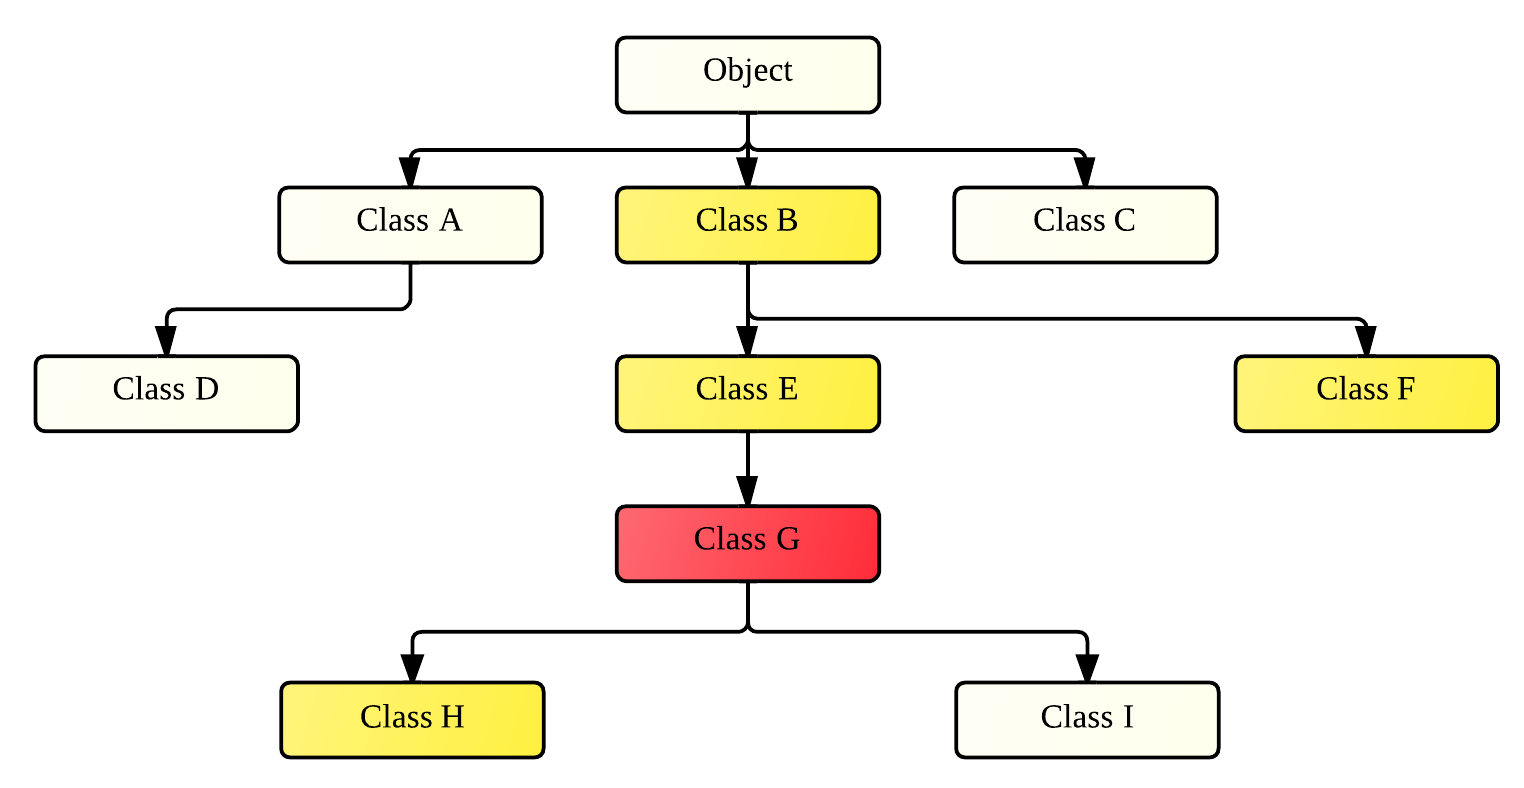
\includegraphics[width=0.7\textwidth]{figs/fig_virtual_call_tree.png}
	}
	\caption{Example class hierarchy; invoked class: $G$, classes implementing the invoked method: $B$, $E$, $F$, $H$}
	\label{fig:TaintPropagation_DestDecision_ClassHierarchy}
\end{figure}

All the other calls rely on dynamic dispatch. Since they are very similar, only the standard \verb$invoke-virtual$ case will be discussed here. By the nature of virtual calls, we know that the invoked method is declared either in the referenced class or in one of its parents, and implemented in any of the children of the declaring class. But not all the implementations of the method can be called by the instruction. In general, these are only implementations in the referenced class, in any of its children, and in the closest parent (only E and H in the example in figure~\ref{fig:TaintPropagation_DestDecision_ClassHierarchy}). If these classes are all internal or all external, the destination of the call is decidable statically. 

Code could be analyzed to further narrow down the number of callable implementations, e.g. by reachability analysis, but it will always be possible to produce code with a statically undecidable call. Then it is necessary to instrument the code so that the decision can be made at runtime. Dexter adds special annotation to every method defined inside the application, which makes internal and external implementations dynamically distinguishable by reflectively finding the target method and checking whether it carries the annotation or not. Slight subtlety comes from the fact that the reflexive API handles public and non-public instance methods differently. Code for non-public methods is shown in listing~\ref{listing:TaintPropagation_MethodCall_DestDecidability_NonPublic}. Instrumentation for public methods uses \verb$Class.getMethod$ to get \verb$m$ and does not need iteration through parents. It is, nonetheless, obvious that these are both very expensive operations. 

One last thing to note is that if an implementation is marked native, it should be considered external regardless of the internality of the containing class
.
\begin{figure}[h]
	\centering
	\begin{tabular}{c}
	\begin{lstlisting}
// original code: obj.methodName(arg1, arg2, ..., argN)
Class c = obj.getClass();
Class[] argTypes = new Class[] { arg1.class, ..., argN.class };

Method m = null;
while (m == null) {
	try {
 		m = c.getDeclaredMethod("methodName", argTypes);
 	} catch (NoSuchMethodException e) {
 		c = c.getSuperclass();
 	}
}

Annotation a = m.getAnnotation(InternalMethodAnnotation.class);
if (a == null) {
	// external call
	obj.methodName(arg1, ..., argN);
} else {
	// internal call
	obj.methodName(arg1, ..., argN);
}
	\end{lstlisting}
	\end{tabular}
	\begin{lstlisting}[caption={Destination-deciding instrumentation for non-public methods},
	                   label={listing:TaintPropagation_MethodCall_DestDecidability_NonPublic}]
	\end{lstlisting}
\end{figure}

\subsection{Internal Method Calls}
\label{section:TaintPropagation_MethodCalls_Internal}

TODO: example?

Method calls identified as internal ought to propagate taint of their arguments into the invoked methods, and taint of their results back to the callers. Since objects carry taint tags globally, only primitive arguments and results require instrumentation. 

Like before, primitives need taint storage. Unfortunately, adding extra parameters is not an option, as the method's prototype could be given by an external interface. Thus, a global integer array is created to hold the taint tags of primitive arguments during a call, and one more global integer variable is created to do the same for a primitive result. To make this thread-safe, each of these stores has a lock that must be acquired before taint is stored, and released once it is not used any more. To get a safer lock-free solution, thread-local storage could be used instead, with the downside of a slightly more complicated instrumentation.

Inside the called method, taint tags of primitive arguments must be retrieved from the global array and assigned to taint registers associated with the registers holding the arguments. But if an internal method is not static or direct, it may also be called from an untrackable, uninstrumented code, in which case the global array would not have been locked or filled, and taint of primitive arguments should be initialized to zero. Every virtual method must therefore be able to recognize whether it was called from an internal or external origin, and handle each case correctly. Since Java programs can read the stack, the name of the caller is easily accessible, and the nature of the origin decidable using reflection. It would be possible to check the annotation of the method, but since the class on the stack is the one that implements the method, one reflexive call was saved by letting Dexter annotate all the internal classes (on top of annotating all the internal methods) and then checking whether this class carries it. 

In the external origin case, instrumentation should also assign the taint of \verb$this$ to all the parameters, including the reference-based ones, provided the method is not static or a constructor. This is useful especially for propagating taint into callbacks, for example in situations like GPS updates, shown in listing~\ref{listing:Source_Location_Listener}. Skipping ahead, \verb$locationManager$ carries location taint and \verb$locationListener$ inherits it when it is passed to the \verb$requestLocationUpdates$ external method. But once its own \verb$onLocationChanged$ method is later called by the service, location taint will be correctly assigned to the parameter using this principle. 

\begin{figure}
	\centering
	\begin{tabular}{c}
	\begin{lstlisting}
LocationManager locationManager = 
  (LocationManager) this.getSystemService(Context.LOCATION_SERVICE);

// define a listener that responds to location updates
LocationListener locationListener = new LocationListener() {
  public void onLocationChanged(Location location) {
    // called when a new location is found 
    // by the network location provider
    useNewLocation(location);
  }

  public void onStatusChanged(
    String provider, int status, Bundle extras) { }

  public void onProviderEnabled(String provider) { }

  public void onProviderDisabled(String provider) { }
};

// register the listener with the Location Manager
locationManager.requestLocationUpdates(
  LocationManager.NETWORK_PROVIDER, 0, 0, locationListener);
	\end{lstlisting}
	\end{tabular}
	\begin{lstlisting}[caption={Example of a location-updating callback class},
	                   label={listing:Source_Location_Listener}]
	\end{lstlisting}
\end{figure}

\subsection{External Method Calls}

TODO: example?

External method calls are the border between trackable and untrackable code, and as such, their instrumentation will have to propagate taint conservatively, accounting for everything that the untrackable code could do. The approach adopted by Dexter is simple - taint of all parameters (including \verb$this$) is combined and assigned to the result and all \emph{mutable} parameters. The assumptions made here are that the method call will always use only data passed to it, and that it can move any of these data to any mutable parameter. In case this proved to cause problematic over-tainting, Dexter offers a way of defining custom policies.

Unfortunately, these assumptions are not safe, as shows the taint-bypassing snippet of code in listing~\ref{listing:ExternalMethodCalls_LogicHole}. It depends on the external environment providing a class that stores data inside invisible fields and then accesses and \emph{leaks} these data. From the Android documentation, it seems that sinks currently identified by Dexter do not have this property. Some combination of framework calls could, however, lead to unidentified leakage. A solution to this problem would be to unify taints of interacting objects, so that tainting \verb$objB$ would automatically taint \verb$objA$, because they interacted on the previous line. But this could easily result in taint explosion.

\begin{figure}[h]
	\centering
	\begin{tabular}{c}
	\begin{lstlisting}
ClassA objA = new ClassA();     // external class
ClassB objB = new ClassB();     // internal class
objA.setX(objB);                // store B inside A
objB.setY(getSensitiveData());  // taint B
objA.useX();                    // use B inside
	\end{lstlisting}
	\end{tabular}
	\begin{lstlisting}[caption={Example of a propagation logic hole},
	                   label={listing:ExternalMethodCalls_LogicHole}]
	\end{lstlisting}
\end{figure}

\subsection{Propagation Logic for Instance Fields}

One implication of the external method call tainting policy is that the method has access to all fields inside passed objects and all elements of passed arrays, and the taint combination must reflect this. It would be possible to iterate through each field and acquire taint separately, but this would be complicated for private fields and could prove extremely slow. Instead, instructions assigning to instance fields are instrumented to propagate taint to the containing object, so that the combined taint can be created only by acquiring its taint tag. Internal fields also have separate taint storage to store their own subset of object taint, but external ones do not because their value could be overwritten by untrackable code which would not update the taint anyway.

\subsection{Sources}

With the taint-propagating infrastructure ready, we can have a look at how access to sensitive data is identified. This varies between sources, but we identified three major use patterns that require different instrumentation, and used these to implement support for six sources (see table~\ref{table:TaintTagStorage_BitMeaning}).

\subsubsection{Database Queries}

First group of sources uses SQL-like queries to access the contact list, recent calls, text messages and other data made available through the interface. Programs call the \verb$ContentResolver.query$ method, passing it a resource identifier (URI) and projection, selection and sorting criteria. The method returns an instance of the \verb$Cursor$ class, which is an iterator through the rows of the query's outcome. 

The type of the source is given entirely by the URI argument, which is merely a textual address. Hence, Dexter only needs to insert a series of \verb$if$ statements that compare the first argument against a list of recognized URIs, and assign the right taint tag to \verb$Cursor$ if a match is found.

\begin{figure}[h]
	\centering
	\begin{tabular}{c}
	\begin{lstlisting}
ContentResolver cr = context.getContentResolver();
URI uri = ContactsContract.Contacts.CONTENT_URI;

`\hl{String uriString = uri.toString();~~~~~~~~~~~~~~~~~~~~~~~~~}`
`\hl{int uriTaint;~~~~~~~~~~~~~~~~~~~~~~~~~~~~~~~~~~~~~~~~~~~~~~}`
`\hl{if (uriString.startsWith("content://com.android.contacts"))}`
`\hl{~~uriTaint = TAINT\_SOURCE\_CONTACTS;~~~~~~~~~~~~~~~~~~~~~~~~}`
`\hl{else if (uriString.startsWith("content://sms"))~~~~~~~~~~~~}`
`\hl{~~uriTaint = TAINT\_SOURCE\_SMS;~~~~~~~~~~~~~~~~~~~~~~~~~~~~~}`
`\hl{else if (uriString.startsWith("content://call\_log"))~~~~~~~}`
`\hl{~~uriTaint = TAINT\_SOURCE\_CALL\_LOG;~~~~~~~~~~~~~~~~~~~~~~~~}`
`\hl{else~~~~~~~~~~~~~~~~~~~~~~~~~~~~~~~~~~~~~~~~~~~~~~~~~~~~~~~}`
`\hl{~~uriTaint = 0;~~~~~~~~~~~~~~~~~~~~~~~~~~~~~~~~~~~~~~~~~~~~}`
Cursor cursor = cr.query(uri, null, null, null, null);
`\hl{TaintMap.set(uriTaint, cursor);~~~~~~~~~~~~~~~~~~~~~~~~~~~~}`

int colName = cursor.getColumnIndex(ContactsContract.Contacts.DISPLAY_NAME);

List<String> contactList = new List<String>();
while (c.moveToNext()) {
	contactList.add(cursor.getString(colName));
}
	\end{lstlisting}
	\end{tabular}
	\begin{lstlisting}[caption={Contact database query, with source instrumentation},
	                   label={listing:Source_DatabaseQuery}]
	\end{lstlisting}
\end{figure}

\subsubsection{System Services}

Information about the operating system and access to hardware resources is provided through the \verb$Context.getSystemService$ method call, which takes one argument, the name of the requested service, and returns a manager object. Complete list of available services can be found in the Android documentation\footnote{\url{https://developer.android.com/reference/android/content/Context.html\#getSystemService(java.lang.String)}}.

Instrumentation for system services is very similar to that of database queries. Name of the requested service is analyzed and the returned object tainted if necessary. Consequently, every piece of data retrieved from the manager will get tainted by the taint propagation logic. 

\begin{figure}[h]
	\centering
	\begin{tabular}{c}
	\begin{lstlisting}
String serviceName = Context.LOCATION_SERVICE;

`\hl{int managerTaint;~~~~~~~~~~~~~~~~~~~~~~~}`
`\hl{if (serviceName.equals("location"))~~~~~}`
`\hl{~~managerTaint = TAINT\_SOURCE\_LOCATION;~}`
`\hl{else if (serviceName.equals("phone"))~~~}`
`\hl{~~managerTaint = TAINT\_SOURCE\_DEVICE\_ID;}`
`\hl{else~~~~~~~~~~~~~~~~~~~~~~~~~~~~~~~~~~~~}`
`\hl{~~managerTaint = 0;~~~~~~~~~~~~~~~~~~~~~}`
Object manager = this.getSystemService(serviceName);
`\hl{TaintMap.set(managerTaint, manager);~~~~}`

LocationManager locationManager = (LocationManager) manager;
Location location = 
  locationManager.getLastKnownLocation(LocationManager.GPS_PROVIDER);
	\end{lstlisting}
	\end{tabular}
	\begin{lstlisting}[caption={Code accessing last known GPS location, with source instrumentation},
	                   label={listing:Source_Location}]
	\end{lstlisting}
\end{figure}

\subsubsection{Browser}

Last category of sources had to be created because of the way browser data are accessed. Even though they are read from a \verb$Cursor$ object, this object is not created by the \verb$ContentResolver.query$ method, but rather by static methods inside class \verb$Browser$. Instrumentation is trivial - insert browser taint assignment after every such method call.

\begin{figure}[h]
	\centering
	\begin{tabular}{c}
	\begin{lstlisting}
ContentResolver cr = context.getContentResolver();

Cursor cursor = Browser.getAllBookmarks(cr);
`\hl{TaintMap.set(TAINT\_SOURCE\_BROWSER, cursor);}`

while (cursor.moveToNext()) {
  ...
}
	\end{lstlisting}
	\end{tabular}
	\begin{lstlisting}[caption={Code accessing browser bookmarks, with source instrumentation},
	                   label={listing:Source_Browser}]
	\end{lstlisting}
\end{figure}

\subsection{Sinks}

The aim of sink instrumentation is to check whether specific API methods, which are known to transfer data out of the application, are called with tainted arguments. Sinks were divided into two groups based on the required approach.

In the following code examples, the \verb$TAINT_SOURCE$ and \verb$TAINT_SINK$ constants will be used. These are bit masks that correspond to the regions of taint tags reserved for source and sink flags (see table~\ref{table:TaintTagStorage_BitMeaning}).

\subsubsection{Always-leaking API Calls}

Most tracked API calls are easy to handle, because they always leak the data passed to them. Those that were implemented are listed in table~\ref{table:Sinks_AlwaysLeaking}, but more could easily be added.

\begin{table}[h]
	\begin{center}
	\begin{tabular}{|l|l|}
		\firsthline
		\textbf{Name}         & \textbf{Tracked Methods} \\
		\hline
		System logging        & \verb$Log.d$, \verb$Log.v$, \verb$Log.i$, ... \\
		Android IPC           & \verb$Context.sendBroadcast$ and similar \\
		Apache HTTP Client    & \verb$HttpClient.execute$ \\
		\lasthline
	\end{tabular}
	\end{center}
	\caption{Always-leaking sinks supported by Dexter}
	\label{table:Sinks_AlwaysLeaking}
\end{table}

Listing~\ref{listing:Sink_ApacheHTTPClient} shows a piece of code that sends data to a remote server using the Apache HTTP Client, which is included in the Android framework. Thanks to taint propagation rules, \verb$post$ inherits the taint of \verb$data$, and thus, once the \verb$execute$ method is called, all that is left to do is to check whether its tag is non-zero, in which case the user needs to be warned.

\begin{figure}[h]
	\centering
	\begin{tabular}{c}
	\begin{lstlisting}
String data = getSomeData();
List<NameValuePair> pairs = Arrays.asList(new BasicNameValuePair("x", data));
HttpEntity postData = new UrlEncodedFormEntity(pairs);
HttpPost post = new HttpPost("http://www.hackers.com/");
post.setEntity(postData);
DefaultHttpClient client = new DefaultHttpClient();

`\hl{if ((TaintMap.get(post) \& TAINT\_SOURCE) != 0) \{}`
`\hl{ // warn the user~~~~~~~~~~~~~~~~~~~~~~~~~~~~~~}`
`\hl{\}~~~~~~~~~~~~~~~~~~~~~~~~~~~~~~~~~~~~~~~~~~~~~~}`
client.execute(post);
	\end{lstlisting}
	\end{tabular}
	\begin{lstlisting}[caption={HTTP request using the Apache client, with sink instrumentation},
	                   label={listing:Sink_ApacheHTTPClient}]
	\end{lstlisting}
\end{figure}

\subsubsection{I/O Writers}

Unfortunately, situation is more complicated for some of the sinks we want to support, namely I/O build around the \verb$Writer$ abstract class. Listing~\ref{listing:Sink_Socket} shows its typical usage for network communication. The tracked method is \verb$PrintWriter.println$, but checking only the taint of the argument is insufficient. In listing~\ref{listing:Sink_ByteArray}, \verb$Writer$ is created with a \verb$ByteArrayOutputStream$, does not form a sink, and we merely want the taint to propagate into \verb$array$. 

We handle this by setting a flag inside the \verb$Socket$ object's taint tag when it is initialized, i.e. making the \verb$Socket.<init>$ method a source of \verb$TAINT_SINK_SOCKET$ data. This taint propagates into the output stream and eventually into the \verb$Writer$ object. Code inserted for the \verb$println$ method then checks whether the object it is called on carries a sink taint, and only proceeds to checking the taint of the argument if it does.

\begin{figure}[h]
	\centering
	\begin{tabular}{c}
	\begin{lstlisting}
String data = getSomeData();

Socket socket = new Socket("hackers.com", 1234);
`\hl{TaintMap.set(TAINT\_SINK\_SOCKET, socket);}`

OutputStream sos = socket.getOutputStream();
PrintWriter writer = new PrintWriter(sos);

`\hl{if ((TaintMap.get(writer) \& TAINT\_SINK) != 0) \{~~~}`
`\hl{~~if ((TaintMap.get(data) \& TAINT\_SOURCE) != 0) \{~}`
`\hl{~~~~// warn the user~~~~~~~~~~~~~~~~~~~~~~~~~~~~~~}`
`\hl{~~\}~~~~~~~~~~~~~~~~~~~~~~~~~~~~~~~~~~~~~~~~~~~~~~~}`
`\hl{\}~~~~~~~~~~~~~~~~~~~~~~~~~~~~~~~~~~~~~~~~~~~~~~~~~}`
writer.println(data);

writer.close();
	\end{lstlisting}
	\end{tabular}
	\begin{lstlisting}[caption={Writer interface used for network communication, with sink instrumentation.},
	                   label={listing:Sink_Socket}]
	\end{lstlisting}
\end{figure}

\begin{figure}[h]
	\centering
	\begin{tabular}{c}
	\begin{lstlisting}
String data = getSomeData();
ByteArrayOutputStream baos = new ByteArrayOutputStream();
PrintWriter writer = new PrintWriter(baos);

`\hl{if ((TaintMap.get(writer) \& TAINT\_SINK) != 0) \{~~~}`
`\hl{~~if ((TaintMap.get(data) \& TAINT\_SOURCE) != 0) \{~}`
`\hl{~~~~// warn the user~~~~~~~~~~~~~~~~~~~~~~~~~~~~~~}`
`\hl{~~\}~~~~~~~~~~~~~~~~~~~~~~~~~~~~~~~~~~~~~~~~~~~~~~~}`
`\hl{\}~~~~~~~~~~~~~~~~~~~~~~~~~~~~~~~~~~~~~~~~~~~~~~~~~}`
writer.println(data);

writer.close();
byte[] array = baos.toByteArray();
	\end{lstlisting}
	\end{tabular}
	\begin{lstlisting}[caption={Writer interface used to turn data into a byte array, with sink instrumentation.},
	                   label={listing:Sink_ByteArray}]
	\end{lstlisting}
\end{figure}

\section{Requirements Analysis}
look at AdCache

\section{Software Engineering}

\subsection{Approach}

\subsection{Android Genome Project}

\section{Tools}

\subsection{Programming Languages}

\subsection{Software Libraries}

\subsection{Android SDK}

\subsection{Version Control}

\subsection{Evaluation Tools}

\cleardoublepage
\chapter{Implementation}

\begin{figure}
	\centerline{	
		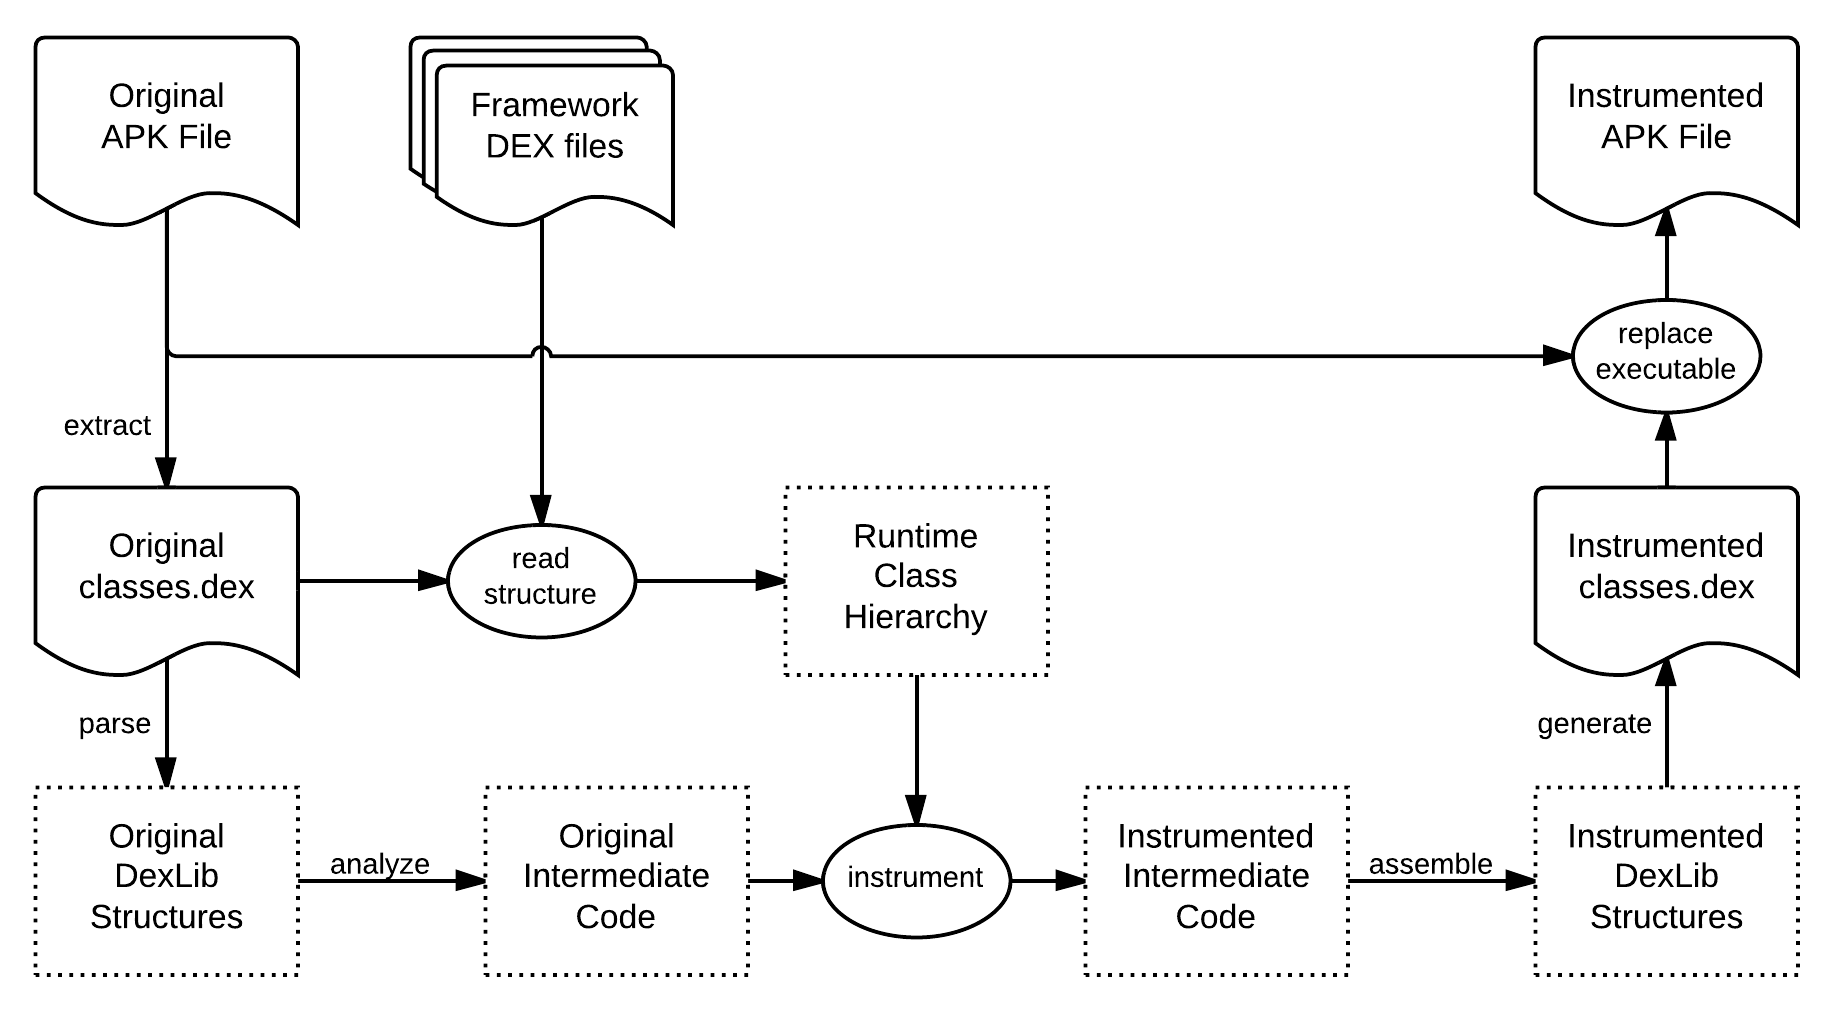
\includegraphics[width=0.9\textwidth]{figs/fig_implementation_overview.png}
	}
	\caption{Schematic diagram of APK instrumentation by Dexter}
	\label{fig:Implementation_Overview}
\end{figure}

Figure~\ref{fig:Implementation_Overview} shows a schematic diagram of all the stages an APK file goes through when given to Dexter to be instrumented. Because of the purpose of some of the stages and the overall pipeline-like linearity of the process, Dexter's architecture resembles one of a compiler. 

The input of the program is the APK file of the application to be instrumented, together with a set of files that form the Android framework, both of which were previously acquired from the user's device. The content of all of these files is parsed to create the complete class hierarchy available to the application at runtime, which will later be of crucial importance for static analysis. The path of the APK file is then evident. The executable \emph{classes.dex} is extracted from the package, parsed and turned into intermediate code, Dexter's internal representation more suitable for analysis and modification than plain assembly. This code is then instrumented according to the rules set out in the previous chapter, reassembled and new executable file generated. By making a copy of the original APK file and replacing the \emph{classes.dex} inside, the final output is created. Since all APKs must be signed, Dexter generates a new signature for the file, using a random key. Each part of this process will be thoroughly explained in the following sections.

\section{Runtime Class Hierarchy}

The purpose of creating a complete picture of the runtime class hierarchy available to the application is being able to reason about the nature of method call destinations, necessary for choosing the correct type of their instrumentation. But class hierarchy is useful in other situations as well, e.g. sources and sinks use class hierarchy to recognize their tracked methods even if the invoking instruction does not reference the expected class but one of its children. To show a concrete example, code in listing~\ref{listing:Sink_ApacheHTTPClient_CanBeApplied} was taken from a method that returns \verb$true$ if and only if given method call should be instrumented as an Apache HTTP Client sink. The tracked \verb$execute$ method is defined in the \verb$HttpClient$ interface, and therefore it can be invoked either using the \verb$invoke-interface$ instruction, referencing the interface as the object type, or using the other two virtual calls, \verb$invoke-virtual$ and \verb$invoke-static$, referencing some class that implements the interface, which is a piece of information that can be provided by the class hierarchy. 

\begin{figure}[h]
	\centering
	\begin{tabular}{c}
	\begin{lstlisting}
val callType = insnInvoke.getCallType();
val invokedClass = insnInvoke.getClassType();
val invokedMethodName = insnInvoke.getMethodName();
val typeHttpClient = DexClassType.parse("Lorg/apache/http/client/HttpClient;", 
                                        parsingCache);

return invokedMethodName.equals("execute") &&
       (
         (
           callType == Opcode_Invoke.Interface && 
           invokedClass.equals(typeHttpClient)
         ) || (
           (callType == Opcode_Invoke.Virtual || 
           	callType == Opcode_Invoke.Super) && 
           `\hl{classHierarchy.implementsInterface(invokedClass, typeHttpClient)}`
         )
       );
	\end{lstlisting}
	\end{tabular}
	\begin{lstlisting}[caption={Code that decides whether a method call given by instruction in \texttt{insnInvoke} should be instrumented as an Apache HTTP Client sink.},
	                   label={listing:Sink_ApacheHTTPClient_CanBeApplied}]
	\end{lstlisting}
\end{figure}

Dexter builds the hierarchy by scanning the application's executable, plus a set of provided framework files. These are all DEX files obtained from the device's \verb$/system/framework$ folder, which contain the classes available at runtime. The framework changes with every new release of Android, and therefore a version compatible with the application must be used, which is the reason why Dexter offers the user to provide their own framework rather than shipping with one particular version. Currently, Dexter also supports scanning JAR files to allow SDK packages to be included in the framework, for example for instrumentation of applications dependent on Google Maps API. But since these SDK packages sometimes do not contain the full class hierarchy, this feature might be dropped and the structure obtained from the respective Android application.

The class hierarchy is a regular tree structure, with each node except the root having exactly one parent, and is implemented as such. Each node contains:
\begin{inparaenum}[(i)]
\item name of superclass,
\item set of children
\item set of implemented interfaces,
\item set of defined methods,
\item set of defined fields,
\item access flags and annotations of the class and its methods and fields.
\end{inparaenum}

All DEX files are parsed by DexLib, its data structures then read and all relevant pieces of information passed to the class hierarchy object. Same is done for JAR files, only these are parsed by the BCEL library. Once all of the files have been scanned, \verb$DexClassHierarchy.checkConsistency$ method is called, which makes sure that:
\begin{inparaenum}[(i)]
\item parent of every class is present,
\item interfaces classes implement are present,
\item interfaces extend \verb$Object$,
\item classes do not implement other classes,
\end{inparaenum}
and creates links between nodes. Every loop-introducing node is rejected during the file-scanning phase.

Class hierarchy provides methods that return pieces of information stored directly in its nodes, or methods that perform simple tree traversal, like returning the set of all ancestors of a class, and hence, there is no point in describing these in greater detail. The only non-trivial method inside this class is the destination-deciding algorithm for method calls, which was already discussed in section~\ref{section:TaintPropagation_DestDecision}. 

It is worth mentioning that method calls can be performed not only on class types but also on arrays. Since their superclass is always \verb$Object$, i.e. they offer methods like \verb$equals$ and \verb$hashCode$, and they are not allowed to override or define methods, Dexter simply treats them as classes of type \verb$Object$. 

\section{Intermediate Code Representation}

Dexter accesses the content of DEX files through the low-level API of DexLib. But the Dalvik VM bytecode, and ultimately the overall structure of the file, was designed so that it could be mapped to memory without any parsing, and code could be executed efficiently. This makes direct instrumentation of the file impossible, because even the smallest modification breaks a multitude of pointers and memory address offsets carefully generated by the JVM-Dalvik conversion tool.

Based on the nature of the instrumentation rules introduced earlier, it would be convenient to represent bytecode of individual methods in a way that constraints would not get broken if:
\begin{inparaenum}[(i)]
\item new instructions were inserted,
\item extra registers were needed,
\item register identifiers did not fit the addressing limits of instructions,
\item different variant of an instruction was used,
\item try blocks overlapped.
\end{inparaenum}
Instrumentation will also necessarily introduce new constants, classes, methods, fields and annotations into the structure of the resulting DEX file, so Dexter needs to create a representation for the whole executable and must be able to convert it back to DexLib's low-level data structures.

\subsection{File Structure}

Classes that represent an executable can be found in the \verb$uk.ac.cam.db538.dexter.dex$ package. Every file is represented by an instance of class \verb$Dex$, which contains a list of \verb$DexClass$ objects that in turn contain lists of \verb$DexMethod$ and \verb$DexField$ objects, etc. Compared to the DexLib classes, these were only designed in a more object-oriented way and thus allow for much easier modification of the file's structure. 

Each of these classes can be created either manually or by passing an instance of the respective DexLib class, which gets recursively parsed. Similarly, each class offers an assembling method that calls itself on all its children in the structure, combines the results and outputs DexLib's representation.

The only part of the file that cannot currently be modified are the values of annotations, simply because this feature was not needed. Values of existing annotations are copied over, but only annotations without values can be added. 

\subsection{Executable Code}

Bytecode of non-abstract and non-native methods is held in instances of the \verb$DexCode$ class. To provide support for the modifications above, the executable code is represented as a list of code elements. These are mostly Dalvik instructions, but they can be interleaved with special markers that represent points in the bytecode originally pointed to by absolute or relative addresses.

\subsubsection{Instructions}

Intermediate instructions used by Dexter group together all semantically equivalent variants of instructions supported by Dalvik. Since they use register objects instead of numerical identifiers, and instead of relative offsets in the code, they store references to the respective markers, they have no addressing limits like their ordinal counterparts. Same applies to pointers into other sections of the executable file, which are replaced with references to objects representing types or various constants. 

Each instruction must also implement methods that provide pieces of information necessary for algorithms that work with executable code. Some of these include:
\begin{inparaenum}[(i)]
\item lists of referenced and defined register arguments,
\item register types before and after the instruction is executed,
\item register identifier range constraints of the least optimized variant,
\item places in the code the interpreter might jump to afterwards.
\end{inparaenum}
Instructions also support replacement of their registers based on provided register-register mapping, which can also be applied only on referenced, defined or both sets of arguments.

\subsubsection{Markers}

Markers specify points inside the executable code that are referred to by instructions or other structures that effect the flow of computation. The supported markers are:
\begin{itemize}
\item \textbf{labels} \\
Labels mark the targets of all branching and \verb$goto$ instructions. They do not carry any special information.
\item \textbf{try/catch blocks} \\
In DEX, try blocks are stored separately from the bytecode. Each block is defined by the absolute addresses of its starting and ending points inside the code. These are replaced by \verb$DexTryBlockStart$ and \verb$DexTryBlockEnd$ markers. Each block can then either supply a list of pairs of exception types and respective instructions to jump to when thrown, and/or a single address to be jumped to if the type of the exception does not match any in the list. \verb$DexCatch$ and \verb$DexCatchAll$ markers are inserted instead of these, and the list of targets is stored in the block's starting marker. 
\item \textbf{method beginning} \\
\verb$DexCodeStart$ is a special marker that is inserted at the beginning of each method after it is parsed. It is used to insert the code that handles entering a method at the correct position, since parameter-moving instructions are inserted at the very beginning at an earlier stage (see sections~\ref{section:Code_ParamRegMapping} and~\ref{section:Code_MethodEntering}).

\end{itemize}

By using markers inside of the code, absolute addresses or relative offsets of these points can be determined at the assembly stage, and inserting extra instructions into the code or replacing existing instructions with their different-sized variants does not break any links.

\subsubsection{Pseudoinstructions}
\label{section:Code_Pseudoinstructions}

Pseudoinstructions are a form of grouping several standard instructions. They were introduced because method calls in Dalvik consist of two separate instructions: an invoke instruction that jumps into the called method, and an optional \verb$move-result$ instruction that stores the returned value into a given register. But since the second instruction does not contain information about the called method, they cannot be instrumented separately. For this reason, intermediate code is scanned before the instrumentation and all these instruction pairs replaced with these pseudoinstructions. After instrumentation, they are expanded back. Same approach is necessary for the \verb$filled-new-array$ instruction.

At the same time, pseudoinstructions can simplify the implementation of some of the instrumentation rules, because they can be used as small inline functions. A simple example of this is the \verb$taint-get$ pseudoinstruction which was already introduced in section~\ref{section:TaintTagStorage_Objects}. It is inserted into the code by the instrumentation rules and afterwards expanded to:
	\begin{figure}[H]
		\centerbox{
			\asm{invoke-static TaintMap.get(vObject)} \\
			\asm{move-result vResult}
		}
	\end{figure}
Similar expanding instructions were created for commonly used operations like printing debug information into the system log or checking methods and classes for the presence of the internality-marking annotations.

\section{DEX Parsing}

The generation of the intermediate code representation is mostly trivial, but the vast number of elements of DEX that need to be modifiable by Dexter makes it a tedious task. 

The input APK file is pushed through DexLib that extracts the executable file and parses it. The data structure it produces is passed to the constructor of Dexter's own \verb$Dex$ class which begins the whole process of conversion to the intermediate format by passing the definitions of individual classes to the constructor of \verb$DexClass$, waiting for it to recursively convert the lower layers of the file structure and then storing the resulting object to a class list. Conversion of all the other layers is similarly straightforward. Encountered pointers are followed into the constant pools of type identifiers, annotations, etc. to store data directly in the nodes together with relevant information found straight in the data structure, and children representing the lower layers of the file are delegated further. 

During the conversion of Dalvik instructions to the intermediate ones, the address of every original instruction is stored with its new counterpart, and all newly introduced marker objects are stored in a separate list together with the address of the instruction they should be inserted in front of. Once the complete instruction list has been created, markers are inserted into their respective positions.

\subsection{Parameter Registers}
\label{section:Code_ParamRegMapping}

It is worth pointing out that a first code modification is applied in this stage, which later simplifies the process of register allocation by removing one of the constraints the algorithm needs to satisfy. It is the fact that every Dalvik method with parameters accesses them through a set of virtual registers with identifiers at the end of the register spectrum it allocates, e.g. a method with seven registers and three parameters accesses them through registers \verb$v4$, \verb$v5$ and \verb$v6$ until it overwrites their values. 

Dexter deals with this by creating a set of registers only for the actual parameters, inserting \verb$move$ instructions at the beginning of the method to copy the values into the correct registers used by the bytecode, and later explicitly allocating these at the end of the spectrum. This way, register allocation can assign identifiers to the regular registers regardless of this requirement. 

\section{Instrumentation}

Once the executable is parsed and converted, all the modifications laid out in the preparation chapter can be applied to it. This is when all the effort put into converting the whole DEX to an intermediate data structure pays off, because the code for application of the instrumentation rules becomes simple and elegant. 

Instrumentation of individual elements is carried out by their respective data structures, e.g. an instance of class \verb$DexField$ that represents an internal field of primitive type creates a new field of type \verb$int$ inside the same class to hold its taint tag, making sure that its name will not conflict with a name of an existing field. 

The process of instrumentation starts by calling the \verb$instrument$ method of the root \verb$Dex$ object, which sets up the environment and delegates the work to its \verb$DexClass$ children. The children pass around an instance of \verb$DexInstrumentationCache$ through which they share common information, like the names of the introduced taint fields.

\subsection{Auxiliary Classes}

While a majority of the newly introduced code is generated based on the content of the file, some of it is always inserted in the same form. This common code includes:
\begin{inparaenum}[(i)]
\item the object taint map,
\item the global array and variable for internal method call taint propagation,
\item internality-marking annotations,
\item taint flag constants,
\item methods analyzing arguments of sources.
\end{inparaenum}

These classes could be generated the same way as the rest of the instrumentation, directly as intermediate code, but for better code clarity, they were implemented in regular Java. Their source files are compiled and converted into a single DEX file that is distributed with Dexter. During instrumentation, this file is converted into intermediate code as well and the two data structures are merged, effectively statically linking the two files. Again, it is made sure that the names of the linked classes are not in conflict with the preexisting ones, and they are stored in the root \verb$Dex$ object where they can be referenced by the code-generating methods.

\subsection{Bytecode Instrumentation}

The method code level is where the most notable instrumentation work is done. The \verb$DexCode.instrument$ method begins by replacing all instructions that need to be grouped as they cannot be instrumented independently (\verb$invoke$ or \verb$filled-new-array$ + \verb$move-result$) with their respective pseudoinstructions. 

With the code prepared, each (pseudo)instruction is asked to generate its instrumentation and place the extra instructions into the code. Implementation of these generators exactly follows the rules of taint propagation logic laid out in section~\ref{section:DataFlowAnalysis}, and therefore will not be discussed any further. Once these are instrumented, the taint register initializing code (see section~\ref{section:TaintPropagation_MethodCalls_Internal}) is inserted in front of the \verb$START$ marker.

\begin{figure}
	\centering
	\begin{minipage}{0.140\textwidth}
	\begin{footnotesize}
		\asm{TRY\_START\_1} \\
		\asm{...} \\
		\asm{TRY\_START\_2} \\
		\asm{...} \\
		\asm{TRY\_END\_2} \\
		\asm{...} \\
		\asm{TRY\_END\_1}
	\end{footnotesize}
	\end{minipage}
	\begin{minipage}{0.09\textwidth}
	\centering
	$\Rightarrow$
	\end{minipage}
	\begin{minipage}{0.150\textwidth}
	\begin{footnotesize}
		\asm{TRY\_START\_1A} \\
		\asm{...} \\
		\asm{TRY\_END\_1A} \\
		\asm{TRY\_START\_2} \\
		\asm{...} \\
		\asm{TRY\_END\_2} \\
		\asm{TRY\_START\_1B} \\
		\asm{...} \\
		\asm{TRY\_END\_1B}
	\end{footnotesize}
	\end{minipage}
	\caption{Removing nested try blocks by splitting the outer block.}
	\label{figure:Instrumentation_TryBlockSplitting}
\end{figure}

This fully instrumented code, however, might not be valid. Pseudoinstructions are expanded first, but instructions that throw exceptions would also have wrapped themselves in a try block. Had such instruction already been inside one, the code would now contain two nested try blocks, an illegal construct in Dalvik. The solution adopted by Dexter is shown in figure~\ref{figure:Instrumentation_TryBlockSplitting}. The outer try block is split into two smaller blocks that cover the code not covered by the inner block. Comparing this against the example instrumentation of the division instruction in figure~\ref{figure:TaintPropagation_ThrowingInstructions}, we see that the \verb$CATCH_ABC$ marker and the instructions following it end up inside the second part of the split outer block. Thus, if the original instructions throws an exception, it is tainted, rethrown and caught by the try block the instruction was original in, preserving the behaviour of the application. On the other hand, the inner try block must handle \emph{all exceptions} the instruction might throw, otherwise they would not get caught despite the outer block defining a matching handler. Catch-all handlers should therefore be used by default.

\label{section:Code_MethodEntering}

\subsection{Object Taint Map}

It was already explained that the object taint map serves as a function from the set of all object references to integers representing their current taint as the instrumented application is being executed, and that it is one of the auxiliary classes implemented in Java and linked in. The data structure suitable to implement this function is a standard hash table, only it needs to use weak object references, because their presence in the table does not prevent garbage collection.

The Java framework does provide an implementation of such hash table in the \verb$WeakHashMap$ class. However, using an instance of this class could potentially lead to changing the behaviour of the application. The problem is that \verb$WeakHashMap$ calls the \verb$hashCode$ method of the given object to determine the slot its entry should be in, and the \verb$equals$ method to compare it against the objects in the linked list of entries in that slot. Since objects can override the safe default implementations of these methods, insertion of the \verb$taint-get$ and \verb$taint-set$ pseudoinstructions would result in calls to original methods that were not present in the original application, not to mention the fact that these methods could throw exceptions, preventing the taint map from functioning. In addition, overriding \verb$equals$ can render any two objects equal, even if they are not of the same type, which would unify their taint tags and taint could propagate uncontrollably. For all these reasons, a safe version of \verb$WeakHashMap$, which would not call any of the object's methods, had to be implemented. 

Removing the call to the \verb$equals$ method is trivial - reference equality operator \verb$==$ is used instead. The \verb$obj.hashCode()$ call was replaced by \verb$obj.getClass().hashCode()$. The \verb$getClass$ method cannot be overridden as it is declared \verb$final$, making the call safe. It returns an object of type \verb$Class$, which represents the type of \verb$obj$. These are automatically generated by the virtual machine when classes are loaded, and so the method cannot be overridden and always uses the original implementation which returns the address of the \verb$Class$ object in the memory. Unfortunately, this means that all instances of one class type will generate the same hash code and will be stored in the same slot. If this ever proved to be a performance bottleneck, native code could be used to return the address of individual objects, but that would reduce the portability of the solution. 

In its current implementation, the hash table is initialized with 1024 slots and does not support dynamic resizing. It exploits temporal locality by moving entries to the beginning of their respective linked lists whenever they are accessed, and deletes garbage collected entries as it encounters them. Methods are declared \verb$public static$ so that they can be invoked from any place in the application. Data are stored in \verb$private static$ fields.

\section{Reassembling}

The algorithms used in parsing and instrumentation are rather elementary and the only difficulty arises from the number of instructions or file structure elements that need to be dealt with individually. This is not the case for the assembling phase, when the intermediate code is converted back to DexLib's data structures. DexLib will automatically generate constant sections of the file and will replace references to their elements by addresses within the file, but it is up to Dexter to generate bytecode that satisfies all the constraints imposed by Dalvik on it. 

The conversion process mostly comes down to allocating register identifiers in such way that each intermediate instruction will be able to generate a valid Dalvik equivalent. Unfortunately, this is a rather complicated task since instrumentation essentially doubles the number of registers used in the computation and the most frequently used Dalvik instructions only allow 4-bit register identifiers and do not have any less optimized variants. Occasionaly, the insertion of extra instructions will also result in instructions performing a jump not being able to address their target because its offset will simply be too large. In these situations, Dexter must be ready to resolve these issues.

Not foreseeing the complexity of this problem unfortunately led to the necessity to build a nearly full-fledged compiler, which in itself is a very challenging task difficult to achieve within the given time frame of the project.  The algorithms used here are mostly taken from the \emph{Modern Compiler Implementation in Java} textbook, and hence their implementation details will be ommited, except their Dalvik-specific modifications. Since the goal of the project was not to build an efficient Dalvik compiler, basic algorithms with simple heuristics were selected, regardless of the performance of the generated code. 

\subsection{Generic Register Allocation}

Register allocation is an optimization problem of assigning a large number of source code variables to a small number of CPU registers. Same register can be used to hold the value of multiple variables, as long as the variables are not \emph{live} at the same time, i.e. the intervals between storing a value and the last point of reading it back do not overlap. If a solution cannot be found, storage in memory is created for some of the variables and load/store instructions that move the value to/from a designated temporary register are inserted in the program, in order to reduce the number of values that need to be held in CPU registers at the same time. This is called \emph{register spilling}.

\subsubsection{Allocation by Graph Colouring}

Typical compiler reduces register allocation to graph colouring, an NP-complete problem, and solves it using some heuristic, balancing the time complexity of the algorithm with the quality of the generated code. 

The graph in question is called \emph{Clash Graph}. Its nodes represent variables, and two nodes are connected by an edge iff the two respective variables cannot be allocated to the same register. If this graph can be coloured with number of colours less than or equal to the number of available CPU registers, a solution to the isomorphic register allocation has been found and can be easily generated, otherwise some registers need to be spilled. 

A commonly used greedy graph-colouring algorithm, which Dexter adopts with slight modifications that will be explained later, uses a simple heuristic to choose a sensible order in which nodes should be coloured. How it works is described by the flow chart in figure~\ref{fig:Implementation_GraphColouring}. Even though it runs in linear time, it usually yields satisfactory results. The algorithm fails if the number of used colours exceeds the number of available registers, in which case a set of variables to be spilled must be selected. An algorithm for this selection is not presented as Dexter simply chooses a random variable and runs the algorithm again. Compilers use more sophisticated analyses to select an optimal set of variables to spill, usually ones that are least used, and do not require the coulouring algorithm to run multiple times.

\begin{figure}
	\centerline{	
		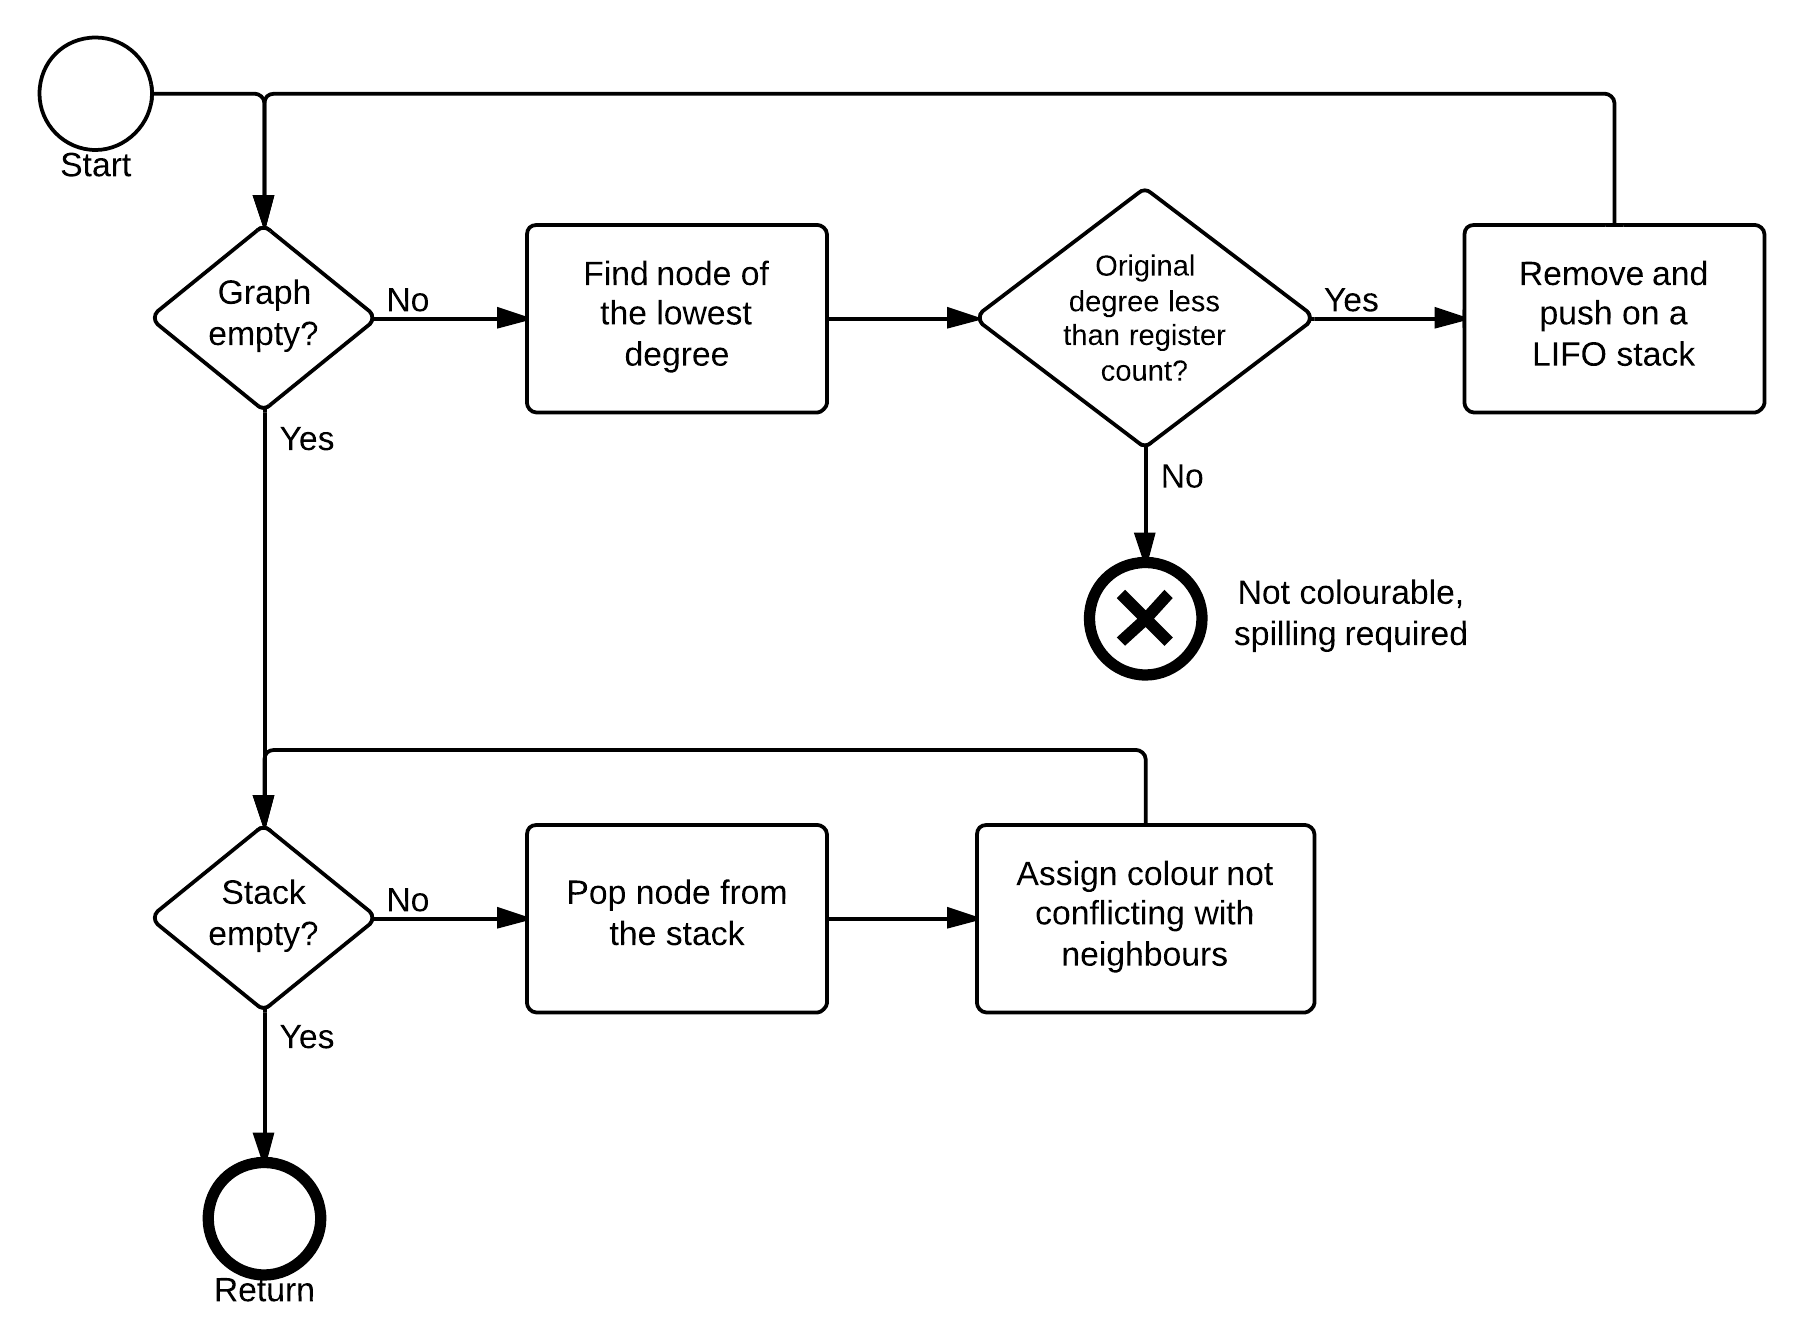
\includegraphics[width=0.9\textwidth]{figs/fig_implementation_gc.png}
	}
	\caption{Flow chart of commonly used greedy graph-colouring algorithm.}
	\label{fig:Implementation_GraphColouring}
\end{figure}

\subsubsection{Building a Clash Graph}

Building a Clash Graph requires comparing the liveness intervals for each variable. This information can be acquired by performing a so-called \emph{Live Variable Analysis} of the program, which requires it to be represented in the form of a \emph{Control Flow Graph}. We will now briefly explain how the CFG of a method is generated and how it is be analyzed.

In CFG, each standard node represents a maximal sequence of instructions, called basic blocks, such that:
\begin{inparaenum}[(i)]
\item each instruction, except possibly the first one, has exactly one predecessor,
\item each instruction, except possibly the last one, has exactly one successor.
\end{inparaenum}
Execution of instructions within a basic block can therefore never unexpectedly leave the block. Nodes $A$ and $B$ are connected by a directed edge iff the execution of last instruction in $A$ can be followed by the execution of first instruction in $B$. For example, an \verb$if$ instruction would always end a basic block and this would be have two successors, since the instruction can either proceed or jump to a label marker. There are also two special nodes, \verb$START$ and \verb$EXIT$, that represent the entry and exit points of the method and are connected to other nodes accordingly.

The principle of CFG generation is not complicated. Each element of the executable code, i.e. both instructions and markers, can specify whether it starts or ends a basic block, whether it can exit the method, and also the complete list of its successors. If it has more than two, it is automatically assumed it ends a block. Code is scanned linearly, instructions put in the current basic block, and new block is created whenever an instruction starting or ending a block is encountered. Blocks are then connected according to the lists of successors of their respective last instructions.

Completeness of the CFG is crutial in order to produce correct liveness intervals of variables and not miss any clashes between variables. A lot of effort therefore had to be invested into reading the (often incomplete) Dalvik documentation to make sure \emph{every} instruction provided a complete list of its successors, reflecting all aspects of the execution semantics, even including the catch blocks the program can jump to if exceptions of various types are thrown. Similarly, instructions throwing exceptions not caught by the surrounding try block must return \verb$true$ when asked whether they can exit the method.

The general idea behind Live Variable Analysis is the propagation of information whether a variable could be read from later in the code to the predecessors. This way liveness analysis produces a list of variables whose values might be needed in the future, for every instruction in the program. The analysis starts by assigning an empty list of variables to every instruction in every node. A loop then iterates through the nodes, always combining the lists of first instructions of all its successors and backwards-propagating the full list through its instructions. A variable is removed from the list if the instruction writes to it, and added if it is referenced. The loop carries on until no more changes are made.

\begin{figure}
	\centerline{	
		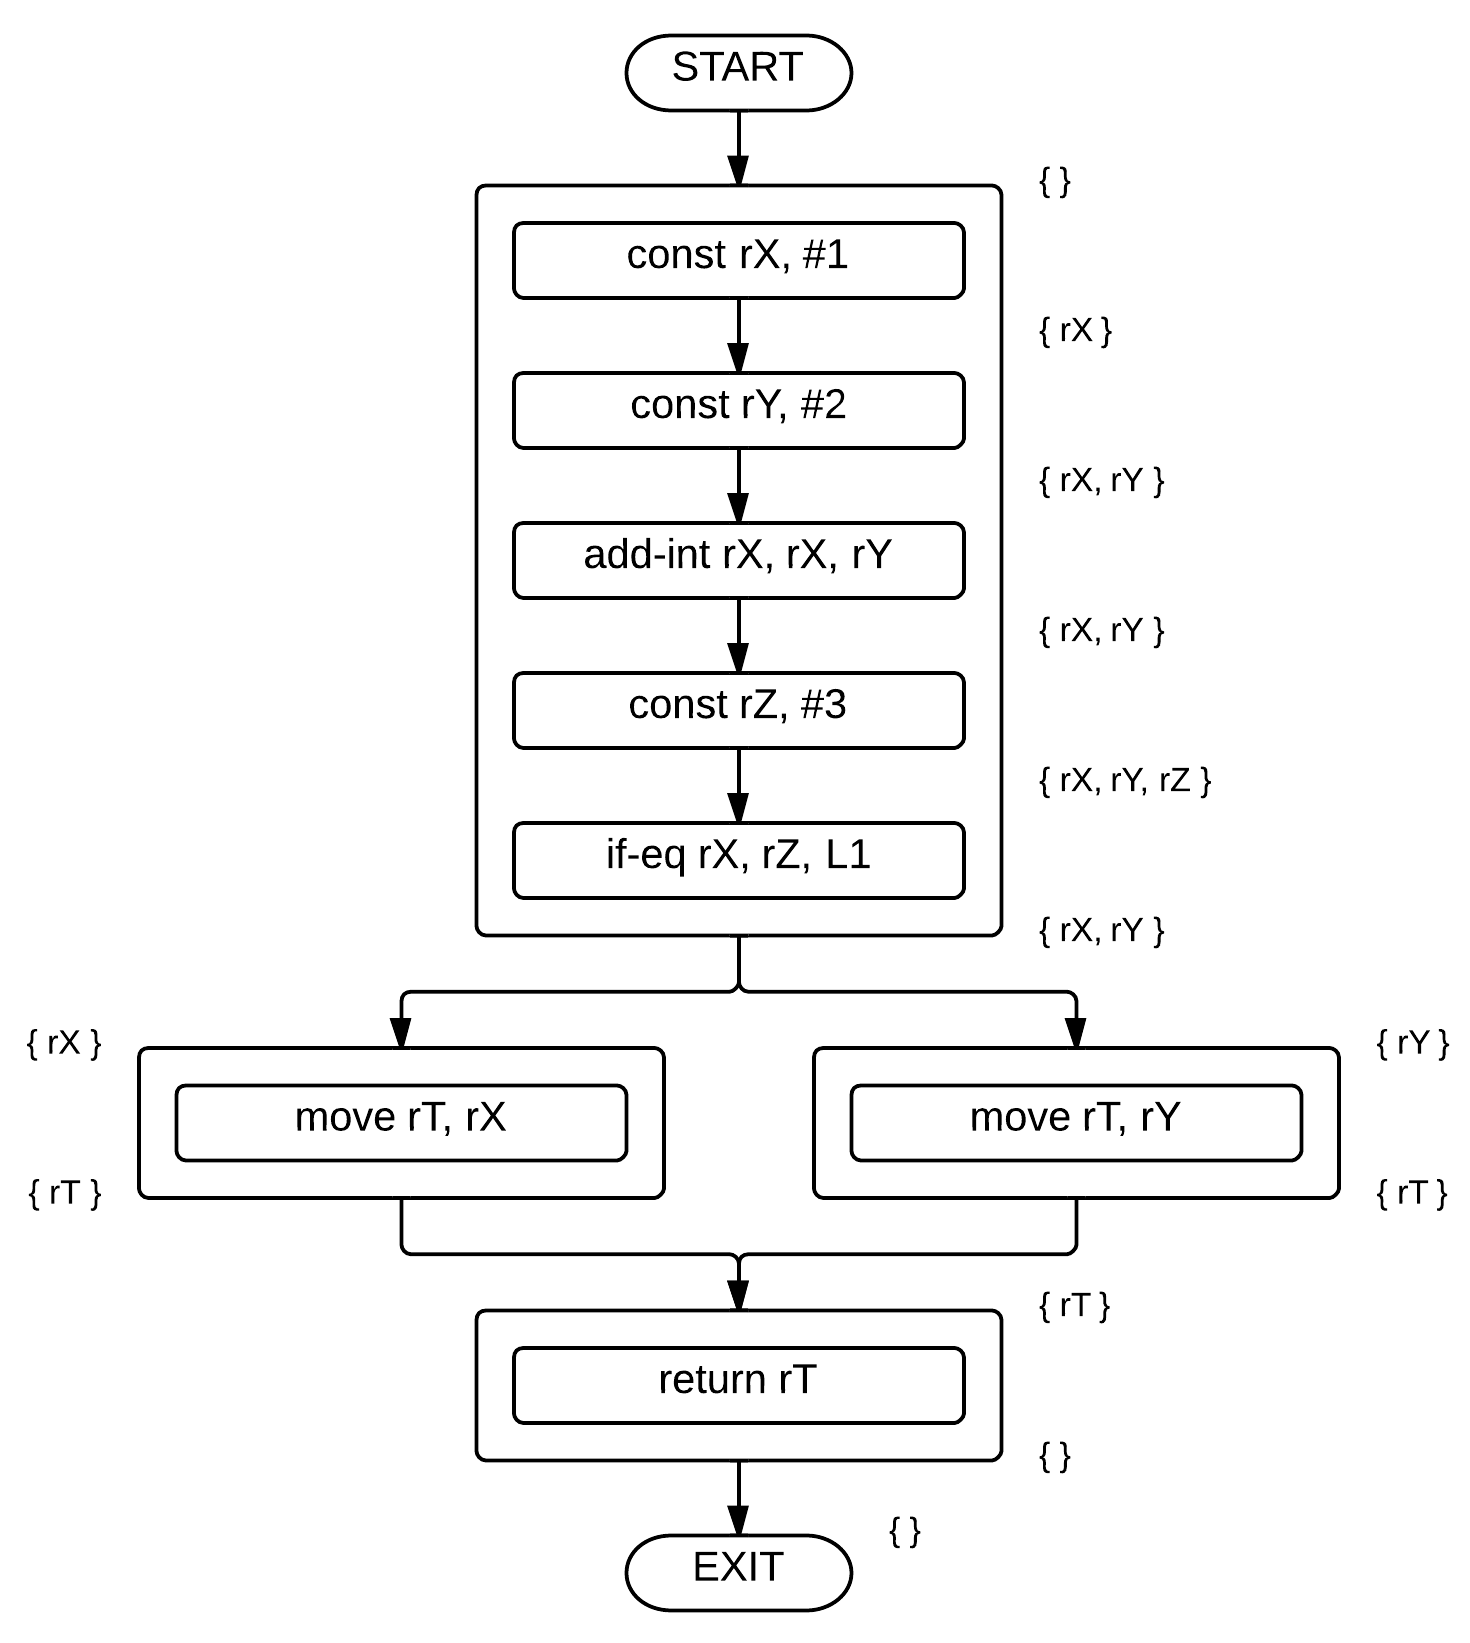
\includegraphics[height=0.42\textheight]{figs/fig_implementation_lva.png}
	}
	\caption{Example of Live Variable Analysis performed on a simple program represented as a Control Flow Graph.}
	\label{fig:Implementation_LVA}
\end{figure}

With the variable lists provided by LVA, generation of the Clash Graph becomes trivial. The algorithm simply iterates through the code and adds an edge for every pair of variables simultaneusly present in the live-variable list of the inspected instruction, as both their values might be required in the future and thus cannot be allocated to the same register. Again, this requires instructions to provide lists of variables they reference and define.

\subsection{Dalvik Register Allocation Specifics}

It is easy to see how the generic register-allocating procedure solves the reassembling problem in Dexter. Register objects inside intermediate code can be thought of as variables used in source code, and these need to be mapped to Dalvik's virtual registers. But due to some constraints imposed on the identifiers, the graph-colouring heuristic requires small alterations, which will be explained in this section.

\subsubsection{Register-Addressing Limits}

The most notable difference is that Dalvik does not differentiate between CPU registers and external memory. Instead, methods are allowed to use up to 65,536 virtual registers, which can be thought of as an equivalent of stack memory, with some of the registers being mapped to the physical registers for efficiency. As we have already seen, most instructions are only capable of addressing the first 16 or 256 registers, and only a limited subset, like the \verb$move$ instructions, can address the rest. 

Instead of checking the degree of the node to identify uncolourable graphs, the graph-colouring algorithm always creates an ordering of nodes and tries to find a non-conflicting colour for each one based on range-limits specified by the intermediate instructions which use the corresponding register object. As not to pollute smaller ranges, colours are first assigned from the higher parts of the spectrum, so for example for node restricted to the 0-255 range a colour in 16-255, not conflicting with the already coloured clashing registers, will be seeked first, and the full 0-255 range will be used only if the former fails. If a valid mapping is found, the identifier spectrum is compacted and mapping returned.

\subsubsection{Consecutive-Identifier Constraints}

Some Dalvik instructions reference registers that are not specified inside the bytecode representation. For example instructions operating with 64-bit values that are stored in register pairs, require these to have consecutive identifiers since they explicitly address only the first register of each pair. There are also \verb$/range$ variants of the \verb$invoke$ instructions which are used to call methods with more than five arguments. These address consecutive registers by specifying the identifier of the first one and their count.

Intermediate instructions reference all register objects explicitly and provide information about their allocation constraints. Dexter acquires these before the graph colouring, checks that they are not in conflict with each other, and builds so-called \emph{node runs} - sequences of one or more Clash Graph nodes that must be assigned consecutive colours. These are built by putting each node in its own linked list, and joining them according to the provided constraints. The order-generating part of the graph-colouring algorithm is modified to find which run the node with lowest degree belongs to, pushing the node run on the stack and removing all its nodes from the graph. The stack-popping loop then needs to be changed to operate on node runs instead. It acquires the addressing limits for each individual register, finds a non-conflicting colour for the first one and checks whether the rest of the run can be assigned the following colours. This is repeated until a valid colouring is found, or until all colours are tried.

\subsubsection{Register Spilling}

As was mentioned previously, register spilling is the process of creating a stack storage for a variable and inserting load/store instructions that move that value to/from CPU registers, in order to reduce the number of values that need to be in registers simultaneously. Since Dalvik programs do not have access to the memory, the equivalent of register spilling is inserting \verb$move$ instructions that transfer data between the designated register and new temporary ones before and after every instructions that uses it, in order to remove some of the constraints imposed on the original intermediate register. Note that because of the consecutive-identifier constraints other nodes in the respective node run needs to be spilled as well.

\begin{figure}
	\centering
	\begin{minipage}{0.325\textwidth}
	\begin{footnotesize}
		\asm{int-to-long rA1 | rA2, rB} \\
		\asm{...} \\
		\asm{int-to-long rA2 | rA3, rC}
	\end{footnotesize}
	\end{minipage}
	\begin{minipage}{0.09\textwidth}
	\centering
	$\Rightarrow$
	\end{minipage}
	\begin{minipage}{0.465\textwidth}
	\begin{footnotesize}
		\asm{move-wide pTemp1 | pTemp2, rA1 | rA2} \\
		\asm{int-to-long pTemp1 | pTemp2, rB} \\
		\asm{move-wide rA1 | rA2, pTemp1 | pTemp2} \\
		\asm{...} \\
		\asm{move-wide pTemp3 | pTemp4, rA2 | rA3} \\
		\asm{int-to-long pTemp3 | pTemp4, rC} \\
		\asm{move-wide rA2 | rA3, pTemp3 | pTemp4}
	\end{footnotesize}
	\end{minipage}
	\caption{Removing nested try blocks by splitting the outer block.}
	\label{figure:Reassembling_RegisterSpilling}
\end{figure}

An example is shown in figure~\ref{figure:Reassembling_RegisterSpilling}. The first instruction requires \verb$rA1$ to be allocated to range 0-15 and \verb$rA2$ to be in the next register, and the second requires the same for \verb$rA2$ and \verb$rA3$. This results in a three-element node run with first two elements confined to the 4-bit range. If register allocation fails, temporaries can be created and \verb$move$ instructions inserted, which results in three independent runs. The original run \verb$[rA1, rA2, rA3]$ can now be stored in the full 16-bit range. The added \verb$[pTemp1, pTemp2]$ and \verb$[pTemp3, pTemp4]$ runs are allocated more easily because they are short, with only first elements restricted to the 4-bit range, and have only short liveness interval.

When colouring fails, Dexter needs to pick a node run to spill. For the sake of simplicity, it chooses a random one in the range that filled up and caused the colouring to fail. However, at the moment not all runs can be spilled. Since different \verb$move$ instructions need to be used for different value types, and registers can hold a value of any type, a type inference algorithm would have to be implemented. Currently, instructions return the type of their arguments, but there are four instructions that cannot do this. These are \emph{if (not) equal (zero)} instructions that are used with both primitives and references. 

\subsection{Static Single-Assignment Form}

\subsection{DexLib Structure Generation}

\section{APK Utilities}

Apk class

\section{User Interface}



\cleardoublepage
\chapter{Evaluation}


\cleardoublepage
\chapter{Conclusion}



\cleardoublepage

%%%%%%%%%%%%%%%%%%%%%%%%%%%%%%%%%%%%%%%%%%%%%%%%%%%%%%%%%%%%%%%%%%%%%
% the bibliography

\addcontentsline{toc}{chapter}{Bibliography}
\bibliography{refs}
\cleardoublepage

%%%%%%%%%%%%%%%%%%%%%%%%%%%%%%%%%%%%%%%%%%%%%%%%%%%%%%%%%%%%%%%%%%%%%
% the appendices
\appendix

\chapter{Latex source}

\section{diss.tex}
{\scriptsize\verbatiminput{diss.tex}}

\section{proposal.tex}
{\scriptsize\verbatiminput{proposal.tex}}

\section{propbody.tex}
{\scriptsize\verbatiminput{propbody.tex}}



\cleardoublepage

\chapter{Makefile}

\section{\label{makefile}Makefile}
{\scriptsize\verbatiminput{makefile.txt}}

\section{refs.bib}
{\scriptsize\verbatiminput{refs.bib}}


\cleardoublepage

\chapter{Bytecode for the Dalvik VM}

% \input{dalvik-bytecode}


\cleardoublepage

\chapter{Project Proposal}


% Draft #1 (final?)

\vfil

\centerline{\Large Computer Science Project Proposal}
\vspace{0.4in}
\centerline{\Large How to write a dissertation in \LaTeX\ }
\vspace{0.4in}
\centerline{\large M. Richards, St John's College}
\vspace{0.3in}
\centerline{\large Originator: Dr M. Richards}
\vspace{0.3in}
\centerline{\large 14$^{th}$ October 2011}

\vfil


\noindent
{\bf Project Supervisor:} Dr M. Richards
\vspace{0.2in}

\noindent
{\bf Director of Studies:} Dr M. Richards
\vspace{0.2in}
\noindent
 
\noindent
{\bf Project Overseers:} Dr~F.~H.~King  \& Dr~A.~W.~Moore


% Main document

\section*{Introduction, The Problem To Be Addressed}


Many students write their CST dissertations in \LaTeX\ and
spend a fair amount of time learning just how to do that. The purpose of 
this project is to write a demonstration dissertation that explains in
detail how it done.  

This core proposal document will be augmented by a separately-printed
cover sheet at the front and a resource form at the end.  Additional
sheets for risk assessment and human resources may also need to be included.

This document will repeat much of the material that is summarised on the additional sheets.

\section*{Starting Point}

{\em Describe existing state of the art, previous work in this area, libraries and databases to be used.
Describe the state of any existing codebase that is to be built on.  }

I am already able to write prose using the English language. I have an online dictionary. etc..

\section*{Resources Required}

{\em A note of the resources required and confirmation of access.}

For this project I shall mainly use my own quad-core computer that runs Fedora Linux. Backup
will be to github and/or to an SVN repository on an external hard disk that is dumped to writable CD/DVD media.
I have another similar computer to hand should my main machine suddenly fail.
I require no other special resources.

\section*{Work to be done}

{\em Describe the technical work.}

The project breaks down into the following sub-projects:

\begin{enumerate}

\item The construction of a skeleton dissertation with the required 
structure. This involves writing the Makefile and makeing dummy files
for the title page, the proforma, chapters 1 to 5, the appendices and
the proposal.

\item Filling in the details required in the cover page and proforma.

\item Writing the contents of chapters 1 to 5, including examples
of common \LaTeX\ constructs.

\item Adding a example of how to use floating figures and encapsulated
postscript diagrams.

\end{enumerate}

\section*{Success Criterion for the Main Result}


The project will be a success if I have a completed dissertation with the correct chapter
titles and I have achieved my other success criterion, which is to blah ...



\section*{Possible Extensions}

{\em Potential further envisaged evaluation metrics or extensions.}

If I achieve my main result early I shall try the following alternative experiment or method of evaluation ...


\section*{Timetable: Workplan and Milestones to be achieved.}


{\em Perhaps list ten or so  two-week work-packages.}

Planned starting date is 16/10/2011.

\begin{enumerate}

\item {\bf Michaelmas weeks 2-4} Learn to use X. Read book Y. Read papers Z.

\item {\bf Michaelmas weeks 5-6} Do preliminary test of Q.

\item {\bf Michaelmas weeks 7-8} Start implementation of main task A.

\item {\bf Michaelmas vacation} Finish A and start main task B.

\item {\bf Lent weeks 0-2} Write progress report. Generate corpus of test examples. Finish task B.  

\item {\bf Lent weeks 3-5} Run main experiments and achieve working project.

\item {\bf Lent weeks 6-8} Second main deliverable here.

\item {\bf Easter vacation:} Extensions and writing dissertation main chapters.

\item {\bf Easter term 0-2:}  Further evaluation and complete dissertation.

\item {\bf Easter term 3:} Proof reading and then an early submission so as to concentrate on examination revision.

\end{enumerate}


 



\end{document}
